\section{Problem (9)}
	A ball is shot vertically upward from the surface of another planet. A plot of $y$ versus $t$ for the ball is shown in \cref{fig:hw2_problem9},

	\begin{figure}[H]
		\begin{center}
			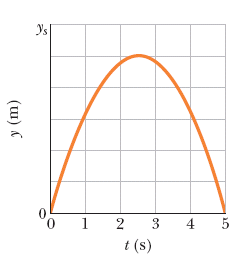
\includegraphics[scale=1]{hw2_problem9}
			\caption{Plot of $y$ versus $t$}
			\label{fig:hw2_problem9}
		\end{center}
	\end{figure}

	where $y$ is the height of the ball above its starting point and $t = 0$ at the instant the ball is shot. The point marked as $y_{s}$ has a value of $48.0 \ m$.

	\subsection{Question (a)}
		What is the magnitude of the free-fall acceleration on the planet?

		\textbf{R:} \newline
		\begin{align}
			y_{s} = \ &48.0 \ m& \notag \\
			y_{i} = \ &\frac{48.0 \ m}{6} = 8 \ m& \notag \\
			y(0 \ s) = \ &0 \ m& \notag \\
			y(1 \ s) \approx \ &25 \ m& \notag \\
			y(2 \ s) \approx \ &38 \ m& \notag \\
			y(2.5 \ s) = \ &40 \ m& \notag \\
			y(3 \ s) \approx \ &38 \ m& \notag \\
			y(4 \ s) \approx \ &25 \ m& \notag \\
			y(5 \ s) \approx \ &0 \ m& \notag
		\end{align}

		\begin{align}
			\bar{v} = \ &\frac{\Delta x}{\Delta t} = \frac{\text{rise}}{\text{run}}& \notag \\
			\bar{v}(0 \ s \to 1 \ s) \approx \ &25 \ m/s& \notag \\
			\bar{v}(1 \ s \to 2 \ s) \approx \ &13 \ m/s& \notag \\
			\bar{v}(2 \ s \to 3 \ s) \approx \ &0 \ m/s& \notag \\
			\bar{v}(3 \ s \to 4 \ s) \approx \ &-13 \ m/s& \notag \\
			\bar{v}(4 \ s \to 5 \ s) \approx \ &-25 \ m/s& \notag
		\end{align}

		\begin{align}
			\bar{a} = \ &\frac{\Delta v}{\Delta t} \notag \\
			\bar{a}(1 \ s \to 2 \ s) \approx \ &-12 \ m/s^{2}& \notag \\
			\bar{a}(2 \ s \to 3 \ s) \approx \ &-13 \ m/s^{2}&  \notag \\
			\bar{a}(3 \ s \to 4 \ s) \approx \ &-13 \ m/s^{2}&  \notag \\
			\bar{a}(4 \ s \to 5 \ s) \approx \ &-12 \ m/s^{2}&  \notag \\
			\text{free-fall acceleration} \approx -12.5 \ m/s^{2}
		\end{align}

	\subsection{Question (b)}
		What is the magnitude of the initial velocity of the ball?

		\textbf{R:} \newline
		\begin{align}
			y = \ &y_{0} + v_{0}t + \frac{1}{2}at^{2}& \notag \\
			25 \ m = \ &(0 \ m) + v_{0}(1 \ s) + \frac{1}{2}\left( -12.5 \ m/s^{2} \right)(1 \ s)^{2}& \notag \\
			v_{0} = \ &\frac{(25 \ m) + (6.25 \ m)}{1 \ s} = 31.25 \ m/s&
		\end{align}

		The function of the \cref{fig:hw2_problem9} can be approximated:

		\begin{align}
			y(t) = 31.25t - 6.25t^{2}
		\end{align}
